\section{Temperature Acquisition Channel}\label{sec:temperatura-acquisition-channel}
	
	Figure \ref{fig:temperature-measurement-block-diagram} shows the solution overview for the thermocouple circuit.

	\begin{figure}[htbp]
		\centering
		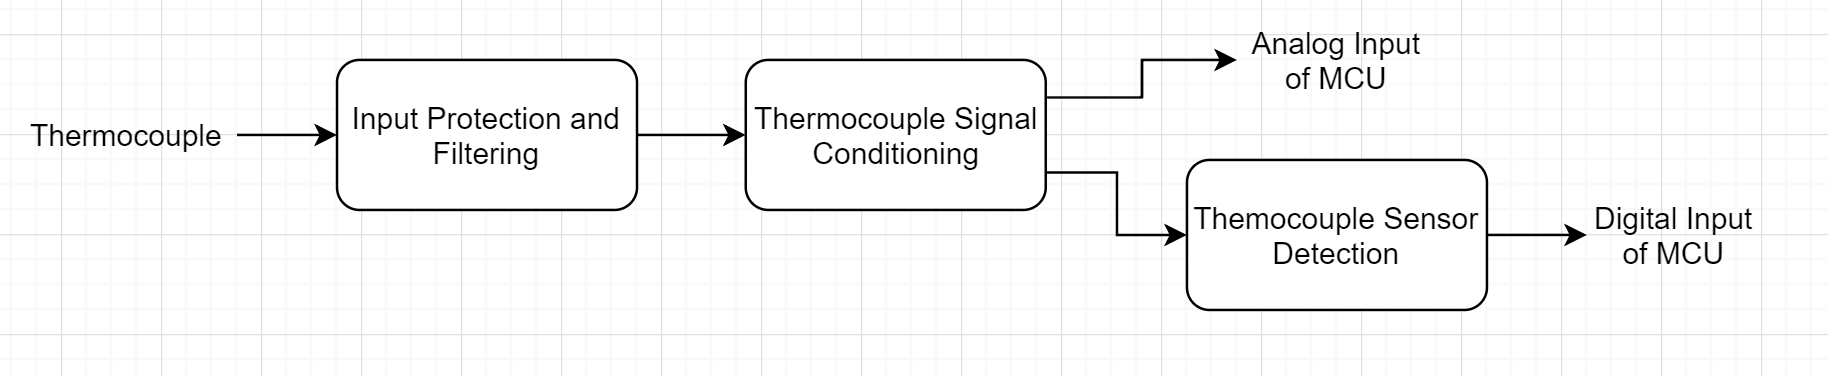
\includegraphics[width=1\textwidth]{figuras/fig-temperature-measurement-block-diagram}
		\caption{Temperature Measurement Block Diagram}
		\label{fig:temperature-measurement-block-diagram}
	\end{figure}

	The function of each block will be explained in the folowing sections.
	
	\subsection{Thermocouple Signal Conditioning}\label{ssec:thermocouple-signal-conditioning}
		
		For this project it was defined that thermocouples of type K (formed by the junction of two metal leagues: Alumel and Cromel) would be used in this project. This is because this specific type of thermocouple has a wide range of operation (-200$^{\circ}$C to 1200 $^{\circ}$C), so according to the requirements they are never too close from the boundary values, a thermocouple of type T or even a type J would not be suitable. Other appealing factor is that this type of thermocouple is quite common so getting eventual replacements would be easier, in comparisson with type E thermocouples.
		\par
		As mentioned in Section \ref{ssec:temperatureMeasurement}, besides amplification and linearization, the thermocouple signal also needs cold junction temperature difference compensation. There is an integrated solution from \textit{Analog Device} called AD8495, this IC functional diagram is displayed on Figure \ref{fig:ad8495-functional-block}.
		
			\begin{figure}[htbp]
				\centering
					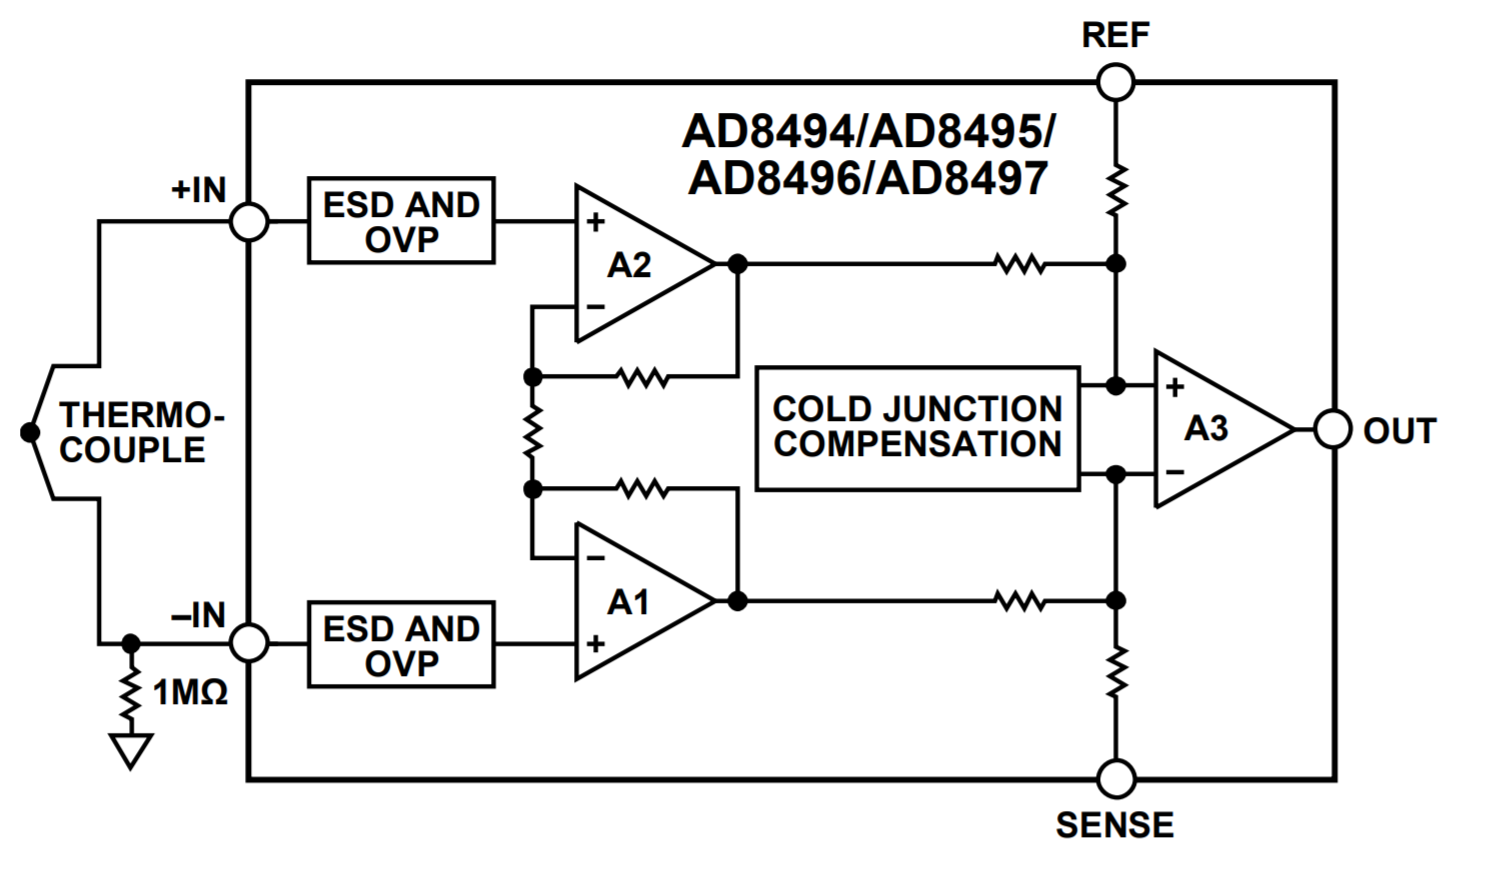
\includegraphics[width=.8\textwidth]{figuras/fig-ad8495-functional-block}
				\caption{AD8495 Functional Block Diagram \cite{ad8495-functional-block}}
				\label{fig:ad8495-functional-block}
			\end{figure}
			
		This IC produces a linearized output with a fixed gain of 5mv/$^{\circ}$C, it is a quite practical solution as it can be powered with single-supply voltage source and it's output saturates to the power supply voltage if the thermocouple is disconnected \cite{ad8495-datasheet}.

	\subsection{Input Protection and Filtering}\label{ssec:ad8495InputProtectionAndFiltering}
	
	Although this IC already has overvoltage and ESD protection, thermocouples tips can pick a load of unwanted noise and transients. Hence, additional protection and external filtering is also recommended by \cite{two-ways-thermocouple}. First thing to do is to add current-limint series resistors, the drawback is doing that is that resistors in the circuit net increases the overall noise. This type of noise is called Johnson-Nyquist Thermal Noise or more commonly just by Johnson Noise, thermal agitation of electrons in a resistor gives rise to random fluctuations in the voltage across its terminals \cite{romero1998johnson}. Moreover, it can be calculated using the following Equation \ref{eqn:johnson-noise} where K is the Boltzmann constant $1.38 \cdot 10^{-23}$, R is the resistance in ohms $(\Omega)$ and T the temperature in kelvin (~300K at room temperature) \cite{sensors2000}.
	
		\begin{equation}\label{eqn:johnson-noise}
			Noise (nv\/\sqrt{Hz}) = \sqrt{4 \cdot K \cdot R \cdot T \cdot 10^{9}}
		\end{equation}
		
	Because the protection circuit includes two equal resistors, whose noise is uncorrelated, that is, the two noise sources are independent of each other—the above result must be multiplied by the square root of 2 (the root sum square of the two noise voltages) and it is considered as a general rule design to tolerate additional Johnson Noise from 10 to 30$\%$ to the amplifier IC \cite{sensors2000}. \cite{two-ways-thermocouple} suggests using current-limiting resistors of 100$\Omega$, according to the AD8495 datasheet \cite{ad8495-datasheet}, the chosen amplifier (AD8495) has a voltage noise density of 32nV$\/ \sqrt{Hz}$. Combining this resistors noise with the amplifier noise will produce an overall noise of 32.485nV$\/\sqrt{Hz}$, which is just 1.5$\%$ above the amplifier's own noise. Additional protection can be achieved using TVS to protect the inputs from differential input overvoltage, considering a bidirectional TVS with a 10V breakdown voltage, the device will theoretically limit the differential voltage between 10V and -10V, the AD8495 has overvoltage protection from -25V to 20V when powered with 5V, so this will help protecting the amplifier inputs. 
	\par
	With the overloads protection done, another important feature to do is to filter undesired signals in the inputs to avoid them to be amplified later, this is done by filtering Radio Frequency Interference (RFI), signal lines (specially for low level signals) are quite susceptible to RF interference \cite{analogDevDesignersGuide}. Interference that occurs on both lines are usually reduced by the amplifiers own CMRR (check Section \ref{itm:opamp-cmrr}), but only on a limited bandwidth, also the in-amp rectifier cannot filter differential RF interference. The chosen amplifier (AD8495) has a -3dB bandwidth at 25kHz, \cite{two-ways-thermocouple} suggests setting a common-mode cutoff filter frequency at 160kHz (in order to guarantee the filter will not attenuate signals inside the 25kHz bandwidth). The standard circuit for the RFI filter is displayed on Figure \ref{fig:rfi-standard-filter}, resistors R and capacitors C$_{C}$ are used to filter common-mode interference. Capacitor C$_{D}$ is connected across the bridge output to reduce any common-mode rejection errors due to the components mismatch, that way filtering any differential interference. C$_{D}$ is usually chosen to be ten times larger than C$_{C}$ \cite{ad8495-datasheet}.
	
		\begin{figure}[htbp]
			\centering
				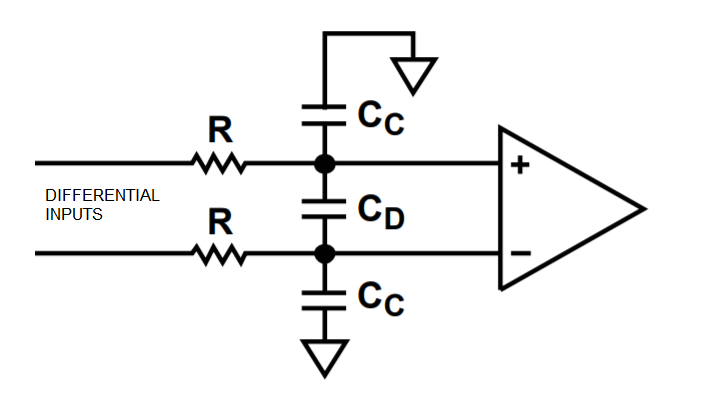
\includegraphics[width=.8\textwidth]{figuras/fig-rfi-standard-filter}
			\caption{RFI}
			\label{fig:rfi-standard-filter}
		\end{figure}

	The -3dB common-mode bandwidth of this filter from Figure \ref{fig:rfi-standard-filter} is given by Equation \ref{eqn:bw-common-mode-rejection-filter} \cite{analogDevDesignersGuide}.

		\begin{equation}\label{eqn:bw-common-mode-rejection-filter}
			BW_{CM}=\frac{1}{2 \cdot \pi \cdot R \cdot C_{C}}
		\end{equation}
	
	The -3dB differential bandwidth of this filter from Figure \ref{fig:rfi-standard-filter} is given by Equation \ref{eqn:bw-differential-rejection-filter} \cite{analogDevDesignersGuide}.
	
		\begin{equation}\label{eqn:bw-differential-rejection-filter}
			BW_{DIFF}=\frac{1}{2 \cdot \pi \cdot R \cdot \left( 2 \cdot C_{C} + C_{d} \right)}
		\end{equation}
		
	Using the values for the current limiting resistors (100$\Omega$), Equation \ref{eqn:bw-common-mode-rejection-filter} and the suggested cutoff frequency of 160kHz \cite{two-ways-thermocouple}, it is possible to calculate a value of 10nF for C$_{C}$. Chosing a C$_{D}$ value ten times larger than C$_{c}$ implies on using a C$_{D}$ value of 100nF, that used on Equation \ref{eqn:bw-differential-rejection-filter} will produce a differential interference filter cutoff frequency of 13kHz.
	\par
	With all this considerations, the Thermocouple Signal Conditioning Circuit can be seen in Figure \ref{fig:temperature-acq-cic}.

	\begin{figure}[htbp]
			\centering
				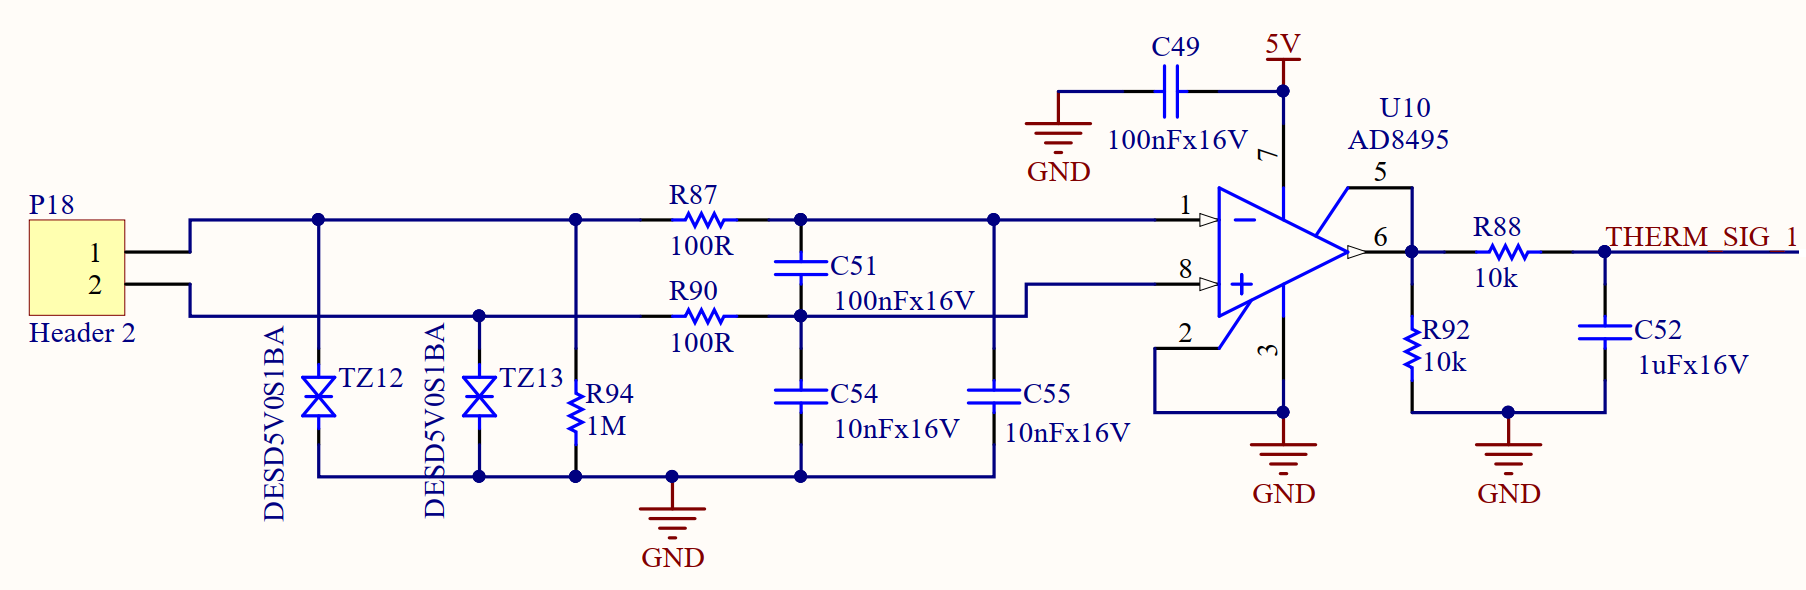
\includegraphics[width=1\textwidth]{figuras/fig-temperature-acq-cic}
			\caption{Thermocouple Signal Conditioning Circuit}
			\label{fig:temperature-acq-cic}
	\end{figure}

	Besides the RFI filter and the amplifier, only a few components were added. First a TVS diode with a standoff voltage of 5V was placed on each of the thermocouple signal tracks. According to \cite{ad8495-datasheet}, in order to implement sensor disconnection detection a 1M resistor should be added to the the thermocouple negative track. More over a post amplification LPF with a cutoff frequency of aproximately 16Hz was placed in order to filter any remain of noise uncorrelated to the thermocouple signal.
		
	\subsection{Thermocouple Sensor Detection}\label{ssec:thermocouple-sensor-detection}
		
	An important feature of any acquisition system is to detect when a sensor is disconnected from the the acquisition system input \cite{o2011pressure}, because a signal acquisition circuit without the signal source will generate outputs that are uncorrelated to what the system was designed to measure/sense on the outside world. The AD8495 has a quite useful feature \cite{ad8495-datasheet}, it offers open thermocouple detection, the inputs of the AD8495 are PNP type transistors, which means that the bias current always flows out of the inputs. This way, the input bias current drives any unconnected output high, which saturates the output to the maximum possible reading, being in this case 1000$^{o}$C or 5V (considering the fixed 5mv/$^{o}$C gain). In Section \ref{sec:functionalRequirements}, it was defined that the system must measure temperatures up to 600$^{o}$C, with the fixed gain of 5mv/$^{o}$ this means an output voltage of 3V. The so called \textit{Thermocouple Sensor Detection} must be able to detect whenever the output exceeds 3V. In order to do that, the circuit displayed in Figure \ref{fig:overvoltage-sensor-detection} was designed.
	
		\begin{figure}[htbp]
			\centering
				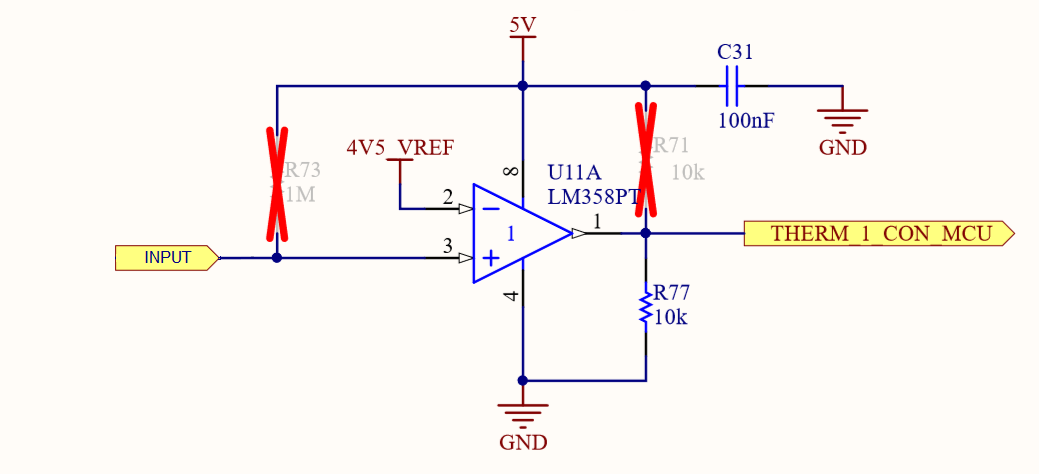
\includegraphics[width=.8\textwidth]{figuras/fig-overvoltage-sensor-detection}
			\caption{Overvoltage Detection Circuit}
			\label{fig:overvoltage-sensor-detection}
		\end{figure}
		
	U11 is an OPAMP working as a comparator, whenever the thermocouple signal is higher than the 4V1 the OPAMP output will saturate to the 5V (the supply voltage applied to the OPAMP). The net 4V1 will be further explained in Section \ref{sssec:4v1-reference}, whereas it is a constant voltage produced on the Power Supplies circuit block. The resistor \textit{R91} is a pull-down resistor used to guarantee that signal will go to low-logic level in case the voltage in the inputs is not present. The capacitors C50 and C53 is just bypass capacitors used to stabilize both the 4V1 and 5V supplies voltage.